\section{Intrinsic challenges of Grid Computing}\label{intrinsic_challenges_of_grid_computing}
While designing a Grid system, intrinsic challenges have to be taken into consideration; that means that \textbf{these challenges exist in Grid Computing independently of the inclusion of mobile devices or operating with just desktop computers}. This section presents a list of the main challenges that a Grid system must face.
\vspace{20mm}

\subsection{Interoperability}
As mentioned in \textit{section \ref{layered_grid_architecture}}, interoperability among any potential participant is the central issue when designing a Grid Architecture, requiring a meticulous focus on designing reliable and versatile protocols for interaction.

Unless the system is designed with the limitation of utilizing a set of identical machines, which is not desirable, machines connected to a Grid operate with \textbf{different hardware}; this differentiation requires a \textbf{layer of abstraction} that separates the functioning of the Grid from the interaction with a single physical node that will use a specific implementation of the standardized Fabric layer.

Anyway, not only do machines offer different hardware, but \textbf{they also differentiate each other in general by the resource they offer}. In the context of distributed execution of computational tasks, for example, nodes offer \textbf{different programming languages} that they are capable of executing. This becomes a problem for interoperability since a requestor might want to execute some task with an implementation in a specific programming language to respect a performance requirement or just because that language offers useful libraries for that particular task. While an implementation of a Fabric layer using a language that is capable of running on almost any device (such as JavaScript) is certainly possible, this creates a great limitation in the Grid's use cases related to distributed computing while at the same time constraining the architecture to a specific technology, which is bad while designing any software.

Obviously, an important interoperability issue comes from the fact that \textbf{nodes can utilize any operating system}, implying different ways of installing the software necessary to run the node's tasks and, most importantly, a differentiation with the interaction with the file system and the security mechanisms specific for that particular OS.

Another resource where nodes differ is the network capabilities that they can offer. Even though this is not a differentiation, in a narrow sense, that comes from the machine in itself but from the environment where it operates, this still becomes an interoperability problem inside a Grid system; for this reason the architecture has to be designed taking into consideration that different nodes will offer \textbf{different levels of reliability and speed for their network connection}, requiring mechanisms for handling errors, disconnections and distributing work accordingly to the network's speed of the node. 

\subsection{Security}\label{security}
Security is an essential prerequisite in every system and the Grid makes no exception. First of all, in order to access to the Grid, it is necessary to have an authentication mechanism (as discussed in section \textit{\ref{connectivity_layer}}); said mechanism must \textbf{uniquely identify every user/entity alongside their unique machines inside the Grid}. While being fundamental in order to grant security, this mechanism is also required by the resources discovery and selection problem (\textit{section \ref{resources_discovery_and_selection}}).

Having a unique identity given by the authentication is also required for another important security problem: respecting resources \textbf{access policies} defined by the nodes providers. Said policies define what resources are offered by a machine, as well as who is authorized to use them. Mechanisms that regulate the enforcement of access policies must also take into consideration the dynamic nature of said policies, since they can be changed by a user at any time.

Unique identification becomes even more important when it is applied to requestors of the services of the Grid. In order to grant the security of volunteers that offer their machines, \textbf{when a user or an entity request a service, it must be trustable (verified) and accountable}. While it is important that also contributors are verified and accountable, this is a lesser concern considering that they can only act as passive entities.

Regarding \textbf{privacy}, once authentication is granted, it is also important that communications among entities inside the Grid are encrypted. The encryption is put in place in order to avoid attacks from malicious entities that could intercept packets.

Finally, countermeasures have to be taken in order to \textbf{avoid the execution of malicious code}; despite the accountability of uniquely identified users helps to reduce this possibility, it is fundamental to implement security measures for avoiding the access to everything that is outside the defined access policies.

\subsection{Scalability, geographical distribution and load balancing}\label{scalabilitu_geographical_distribution_and_load_balancing}
The main strength of the Grid is its ability to scale, becoming a central principle that guides the design of the system. In such a system, it is possible to identify two main contexts where it is necessary to design \textbf{horizontal scalability}:
\vspace{5mm}
\begin{itemize}
    \item \textit{The nodes' context}, i.e. the ability for the system to work with a varying amount of machines offered by volunteers;
    \item \textit{The cloud's context}, i.e. the capability of the cloud architecture to scale in order to support efficiently the nodes' context.
\end{itemize}

It is clear the cloud's context is the foundation of the system, therefore here it is necessary to design a \textbf{load balancing mechanism for the cloud services}, increasing/decreasing the number of machines running such services, depending on the number of nodes that are participating in the Grid in a certain moment.

Moreover, this load balancing has to implement a \textbf{geographically-aware behavior}, since the nodes are scattered around the planet without a fixated location; this results in the necessity of creating new replicas of the cloud services' servers in a geographical location that takes into consideration not only the costs of running such server, but it also \textbf{optimizes the proximity with as many nodes as possible in order to reduce latency}. Once a server is instantiated, it is necessary to let the new instance take charge of the handling of part of the nodes connected to the overloaded service. Vice versa, if there is not an excessive amount of traffic, an instance might be removed and its nodes given to another previously instantiated server.
Since the load balancing introduces a problem of reachability for both the cloud services and the nodes (the dynamically instantiated services with a geographically-aware behavior lack a fixed address), it is also necessary to introduce \textbf{discovery services} that, on the contrary, have a static address and act as intermediaries, providing the address of the required service instances.

\begin{figure}[!ht]
    \centering
    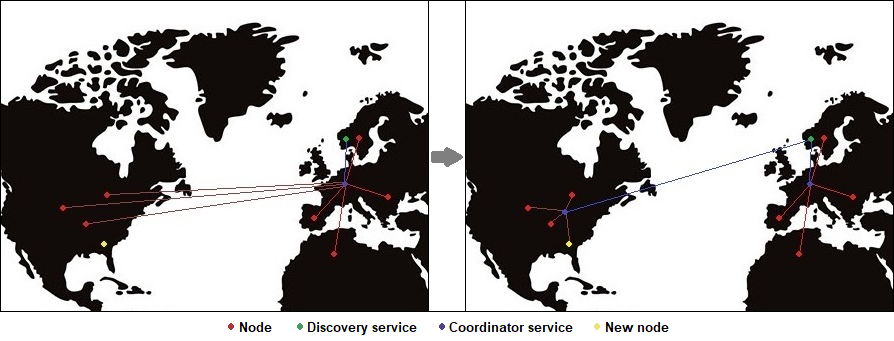
\includegraphics[width=\textwidth]{document/chapters/chapter_2/images/server_instantiation.png}
    \caption{Example of geographically-aware load balancing}
    \label{fig:server_instantiation}
\end{figure}

On a final note, this dynamic instantiation in the nodes' context has to be considered while designing the authentication mechanism (discussed in \textit{section \ref{security}}), requiring for it to work even if something changes with the servers' status.


\subsection{Resources discovery and selection}\label{resources_discovery_and_selection}
Not only does the Collective layer (\textit{section \ref{fig:collective_layer}}) handles global interactions among collections of resources, but, first and foremost, it has the responsibility of managing the discovery of resources and the selection of the correct ones to perform a task.

Cloud services devolved to this duty build a \textbf{map of all the nodes connected to the Grid, keeping track of also which resources they can offer}. With this knowledge, said services can \textbf{connect a requestor to the desired resources}, eventually \textbf{choosing the best fit among multiple possible resources of a certain type} that satisfy the condition for a certain task.

The map of the nodes connected to the Grid has to be designed to be stored in multiple server instances in order to respect the scalability discussed in the previous section.

\subsection{Scheduling, fault tolerance and Quality of Service (QoS)}
An operation that needs to be performed inside the Grid needs a \textbf{scheduling mechanism} in order to handle the execution of said operations. Since the operations are executed in a distributed environment prone to errors, \textbf{replication of data} needs to be performed among multiple nodes; this is done to increase \textbf{fault tolerance} since any node can fail at any moment. Increasing the replication factor to strengthen the tolerance to errors necessarily means a worsening of the performances inside the distributed system and vice versa. The correct replication factor highly depends on the tasks that the Grid needs to perform and how performances are valued compared to availability.

All these factors (along with what discussed in the previous sections) influence the quality of service that the Grid can offer. Every design decision for the Grid has to be made with the intent of \textbf{maximizing the QoS}, increasing performances as much as possible while, at the same time, offering good fault tolerance, scalability, and security.
